\documentclass[12pt]{report}

\usepackage{geometry}
\geometry{a4paper,scale=0.8}

\usepackage{indentfirst}
\usepackage{caption}
\usepackage{graphicx, subfig}

\usepackage{mathrsfs}
\usepackage{float}

\usepackage[BoldFont,SlantFont,CJKchecksingle]{xeCJK}
\setCJKmainfont[BoldFont=STHeitiSC-Light,SlantedFont=STKaitiSC-Regular]{STSongti-SC-Regular}
\setCJKsansfont[BoldFont=STHeitiSC-Light,SlantedFont=STKaitiSC-Regular]{STSongti-SC-Regular}
\setCJKmonofont[ItalicFont={STFangsong}]{STSongti-SC-Regular}
\setCJKfamilyfont{zhsong}{STSongti-SC-Regular}
\setCJKfamilyfont{zhhei}{STHeitiSC-Light}
\setCJKfamilyfont{zhkai}{STKaitiSC-Regular}
\setCJKfamilyfont{zhfs}{STFangsong}

	
\title{马尔科夫场}
	
\author{王方正 21721240}

\date{}

\begin{document}
		
	\maketitle
		
	\tableofcontents
	
	\renewcommand\thesection{\arabic {section}}
		
	\section{模型定义}
	
		马尔科夫随机场,又称为概率无向图模型,是一个可以由无向图表示的联合概率分布。
		
		\subsection{基础定义}
		
			图是由结点及连接结点的边组成的集合。结点和边分别记作$v$和$e$,结点和边的集合分别记作$V$和$E$,图记作$G=(V,E)$。无向图是指边没有方向的图。
		
			概率图模型(PGM)是由图表示的概率分布。设有联合概率分布$P(Y)$,$Y\in\mathcal{Y}$是一组随机变量。由无向图$G=(V,E)$表示概率分布,即在图$G$中,结点$v\in V$表示一个随机变量$Y_v$,$Y=(Y_v)_{v\in V}$;边$e\in E$表示随机变量之间的概率依赖关系。
				
		\subsection{马尔可夫性}
		
			马尔可夫性可分为成对马尔可夫性、局部马尔可夫性和全局马尔可夫性,表达公式如下:
		
			\begin{itemize}
				\item 成对马尔可夫性:$P(Y_u,Y_v|Y_O)=P(Y_u|Y_O)P(Y_v|Y_O)$
				\item 局部马尔可夫性:$P(Y_v,Y_O|Y_W)=P(Y_v|Y_W)P(Y_O|Y_W)$
				\item 全局马尔可夫性:$P(Y_A,Y_B|Y_C)=P(Y_A|Y_C)P(Y_B|Y_C)$
			\end{itemize}
		
			\subsubsection{成对马尔可夫性}	
			
				设$u$和$v$是无向图$G$中任意两个没有边连接的结点,结点$u$和$v$分别对应随机变量$Y_u$和$Y_v$。其他所有结点为$O$,对应的随机变量组是$Y_O$。成对马尔可夫性是指给定随机变量组$Y_O$的条件下随机变量$Y_u$和$Y_v$是条件独立的。
				
			\subsubsection{局部马尔可夫性}
				
				设$v\in{V}$是无向图$G$中任意一个结点,$W$是与$v$有边连接的所有结点,$O$是$v$, $W$以外的其他所有结点。$v$、$W$、$O$分别表示随机变量$Y_v$,以及随机变量组$Y_W$和$Y_O$。局部马尔可夫性是指在给定随机变量组$Y_W$的条件下随机变量$Y_v$与随机变量组$Y_O$是独立的,如Figure 1所示。
	
				\begin{figure}[H]
					\centering
					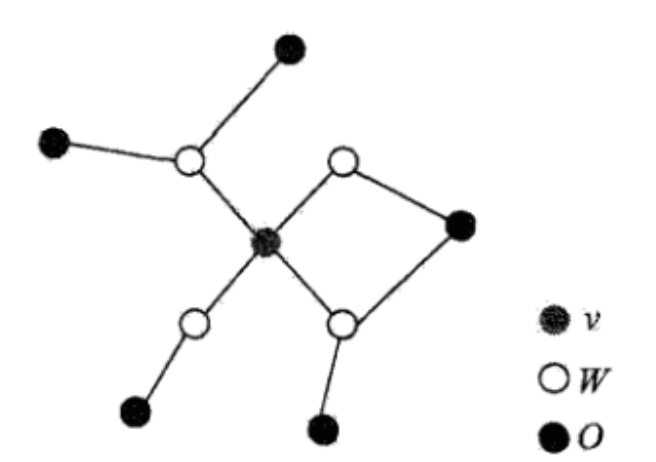
\includegraphics[scale=0.6]{img/1.png}
					\caption{局部马尔可夫性} 
					\label{img}
				\end{figure}
			
			\subsubsection{全局马尔可夫性}
			
				设结点集合$A$,$B$是在无向图$G$中被结点集合$C$分开的任意结点集合,如Figure 2所示。结点集合$A$,$B$和$C$所对应的随机变量组分别是$Y_A$,$Y_B$和$Y_C$。全局马尔可夫性是指给定随机变量组$Y_C$条件下随机变量组$Y_A$和$Y_B$是条件独立的。
				
				\begin{figure}[H]
					\centering
					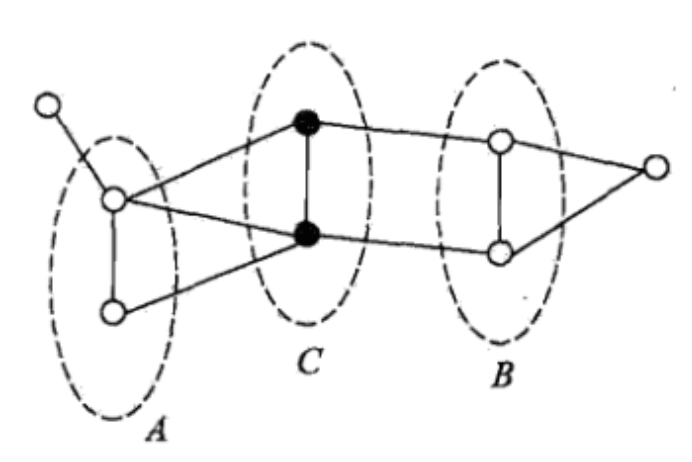
\includegraphics[scale=0.6]{img/2.png}
					\caption{全局马尔可夫性}
					\label{img}
				\end{figure}
			
			上述成对的、局部的、全局的马尔可夫性定义是等价的。
			
		\subsection{模型定义}
			
			设有联合概率分布$P(Y)$ ,由无向图$G=(V,E)$表示,在图$G$中,结点表示随机变量,边表示随机变量之间的依赖关系。如果联合概率分布$P(Y)$满足成对、局部或全局马尔可夫性,就称此联合概率分布为概率无向图模型或马尔可夫随机场。
			
	\section{因子分解}
	
		\subsection{团与最大团}
		
			无向图$G$中任何两个结点均有边连接的结点子集称为团。
		
			若$C$是无向图$G$的一个团,并且不能再加进任何一个$G$的结点使其成为一个更大的团,则称此$C$为最大团。
	
			Figure 3中左图表示由7个结点组成的无向图。图中有3个最大团$\{Y_1,Y_2,Y_3,Y_4\}$、$\{Y_4,Y_5,Y_6\}$和$\{Y_6,Y_7\}$。右图是根据最大图将无向图转化得到的相应的因子图,其中黑结点表示一个最大团,与黑结点相连的其他结点表示在一个最大团中两两相连。
			
			\begin{figure}[H]
				\centering
				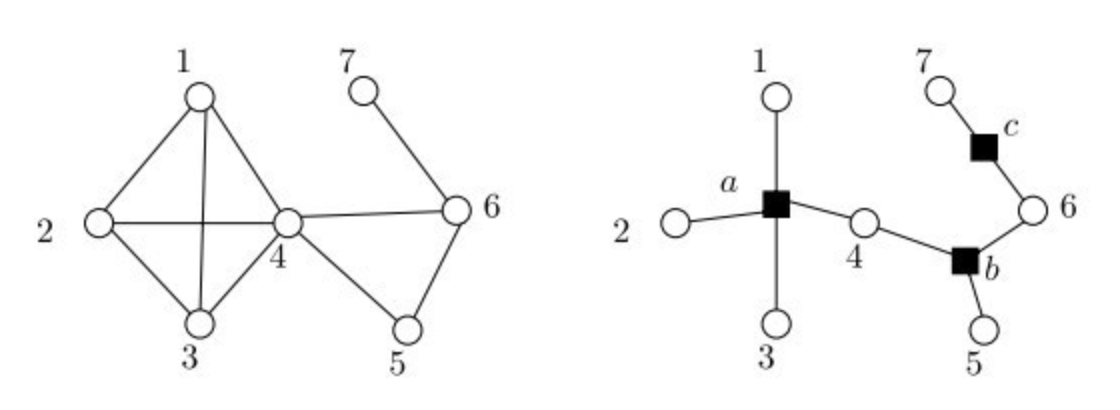
\includegraphics[scale=0.6]{img/3.png}
				\caption{无向图与因子图}
				\label{img}
			\end{figure}
		
		\subsection{因子分解}
		
			将概率无向图模型的联合概率分布表示为其最大团上的随机变量的函数的乘积形式的操作,称为概率无向图模型的因子分解。
			
			给定概率无向图模型,设其无向图为$G$,$C$为$G$上的最大团,$Y_C$表示$C$对应的随机变量,那么概率无向图模型的联合概率分布$P(Y)$可写作图中所有最大团$C$上的函数的乘积形式,具体公式为:
			$$P(Y)=\frac{1}{Z}\prod_{C}\Psi_{C}(Y_C)$$
			其中,Z是规范化因子,由式
			$$Z=\sum_{Y}\prod_{C}\Psi_{C}(Y_C)$$
			给出。规范化因子保证$P(Y)$构成一个概率分布。
			函数$\Psi_{C}(Y_C)$称为势函数,通常定义为指数函数:
			$$\Psi_{C}(Y_C)=exp^{-E(Y_C)}$$
			势函数的作用是刻画变量之间的相关关系,它是非负函数,并且在所偏好的变量取值上有较大函数值。
			
	\section{应用}
	
		\subsection{图像分割}
			
			图像分割是机器视觉领域一个重要的研究方向,是图像分析和理解的基础。在概率框架下,MRF模型较好地描述了图像邻域像素的相似特性,得到了广泛应用。
			
			基于MRF模型的分割方法建立在MRF模型和贝叶斯理论(Bayesian theory)的基础上,根据统计决策和估计理论中的最优准则确定图像分割问题的目标函数,采用一些优化算法求取满足这些条件的MRF的最大可能分布,从而将图像分割问题转换为MRF分布的最优化问题。如Figure 4所示。
			
			\begin{figure}[H]
				\centering
				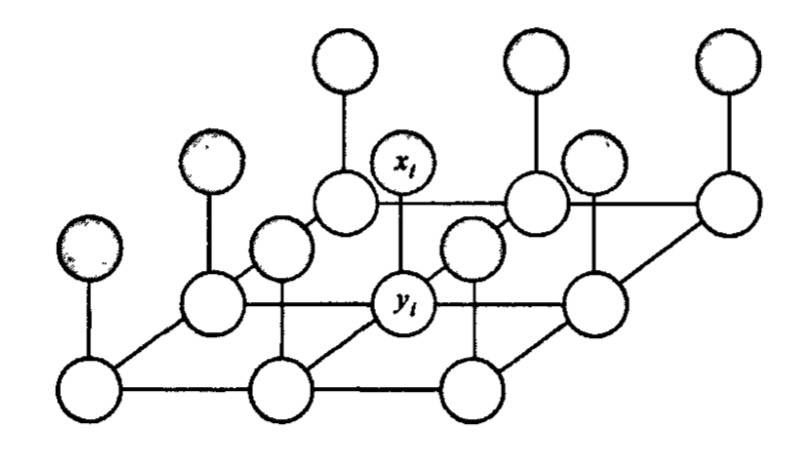
\includegraphics[scale=0.6]{img/4.png}
				\caption{Pairwise MRF 模型}
				\label{img}
			\end{figure}
			
			MRF相比其他方法的优势是:
			
			\begin{itemize}
				\item 提供了一种principled method来对Prior knowledge建模
				\item MRF可以很容易用定量的方法描述contextual information
			\end{itemize}
		
			因此,相比其它pixel-based, 或local-based 方法,它可以考虑到环境知识的影响,如果建立的图模型得当,进而可能获得全局最优解释,这样正是向human vision更靠近了一步。
			
				
\end{document}